% --------------------------------------------------------------
% This is all preamble stuff that you don't have to worry about.
% Head down to where it says "Start here"
% --------------------------------------------------------------
 
\documentclass[12pt]{article}
 
\usepackage[margin=1in]{geometry} 
\usepackage{amsmath,amsthm,amssymb}
\usepackage{gensymb}
\usepackage{graphicx}
 \usepackage{tikz,pgfplots}
\usepackage{float}
\usepackage{enumitem}
\usepackage[utf8]{inputenc}


\newcommand{\N}{\mathbb{N}}
\newcommand{\Z}{\mathbb{Z}}

\newcommand{\slantedgrid}[4]{%
   \pgfmathtruncatemacro{\result}{#1+#3}
   \foreach \x in {#1,...,\result} \draw (\x,#2) -- ++(#4,#4);%
   \pgfmathtruncatemacro{\result}{#2+#4}
   \foreach \y in {#2,...,\result} \draw (#1+\y-#2,\y) -- ++(#3,0);%
 }
 
\DeclareMathOperator\erf{erf}
 
\newenvironment{theorem}[2][Theorem]{\begin{trivlist}
\item[\hskip \labelsep {\bfseries #1}\hskip \labelsep {\bfseries #2.}]}{\end{trivlist}}
\newenvironment{lemma}[2][Lemma]{\begin{trivlist}
\item[\hskip \labelsep {\bfseries #1}\hskip \labelsep {\bfseries #2.}]}{\end{trivlist}}
\newenvironment{exercise}[2][Exercise]{\begin{trivlist}
\item[\hskip \labelsep {\bfseries #1}\hskip \labelsep {\bfseries #2.}]}{\end{trivlist}}
\newenvironment{problem}[2][Problem]{\begin{trivlist}
\item[\hskip \labelsep {\bfseries #1}\hskip \labelsep {\bfseries #2.}]}{\end{trivlist}}
\newenvironment{question}[2][Question]{\begin{trivlist}
\item[\hskip \labelsep {\bfseries #1}\hskip \labelsep {\bfseries #2.}]}{\end{trivlist}}
\newenvironment{corollary}[2][Corollary]{\begin{trivlist}
\item[\hskip \labelsep {\bfseries #1}\hskip \labelsep {\bfseries #2.}]}{\end{trivlist}}
 
\begin{document}
\providecommand{\e}[1]{\ensuremath{\times 10^{#1}}}
\providecommand{\ex}[1]{\ensuremath{10^{#1}}}
% --------------------------------------------------------------
%                         Start here
% --------------------------------------------------------------
 
\title{HW 8}
\author{Levon Dovlatyan \\ SI: 24451582\\ E45} 
\date{Nov 7, 2014}
\maketitle
 
\begin{problem}{8.1} 
Which of the alloys in Table 8.1 would you expect to exhibit ductile-to-brittle transition behavior?  (State the basis of your selection).
\end{problem}
We know from Schackelford that steels go through a ductile-to-brittle transition because their lattice structure is bcc. The only steel alloy in table 8.1 [1] that does not have a bcc structure is 410 stainless steel. We know that stainless steels have a fcc lattice group instead. This means that 1040 carbon steel, 8630 low-alloy steel, and L2 tool steel must go through the ductile-to-brittle transistion [1]. To find out if the other alloys in table 8.1 have a bcc lattice structure, we can look at table 11.1 in sec 11.1 which contains information on a lot of the alloys in table 8.1. From section 11.1, we see that ductile iron and Nb-1 Zr contain bcc lattice structures and must also have a ductile-to-brittle transition [1].
\begin{enumerate}
\item 1040 carbon steel
\item 8630 low-alloy steel
\item L2 tool steel
\item ductile iron, quench
\item Nb-1 Zr
\end{enumerate}

\begin{problem}{8.4}
 The following data were obtained from a series of Charpy impact tests on a particular structural steel. \textbf{(a)} Plot the data as impact energy versus temperature. \textbf{(b)}  What is the ductile-to-brittle transition temperature, determined as corresponding to the average of the maximum and minimum impact energies? 
 \begin{center}
 \begin{tabular}{c | c}
 Temperature($\degree$C) & Impact Energy (J) \\ \hline
100 & 84.9 \\ \hline
60 & 82.8 \\ \hline
20 & 81.2 \\ \hline
0 & 77.9 \\ \hline
-20 & 74.5 \\ \hline
-40 & 67.8 \\ \hline
-60 & 50.8 \\ \hline
-80 & 36.0 \\ \hline
-100 & 28.1 \\ \hline
-140 & 25.6 \\ \hline
-180 & 25.1 \\ \hline
 \end{tabular}
 \end{center}
 \end{problem}

\textbf{(a)}
\begin{figure}[H]
\centering
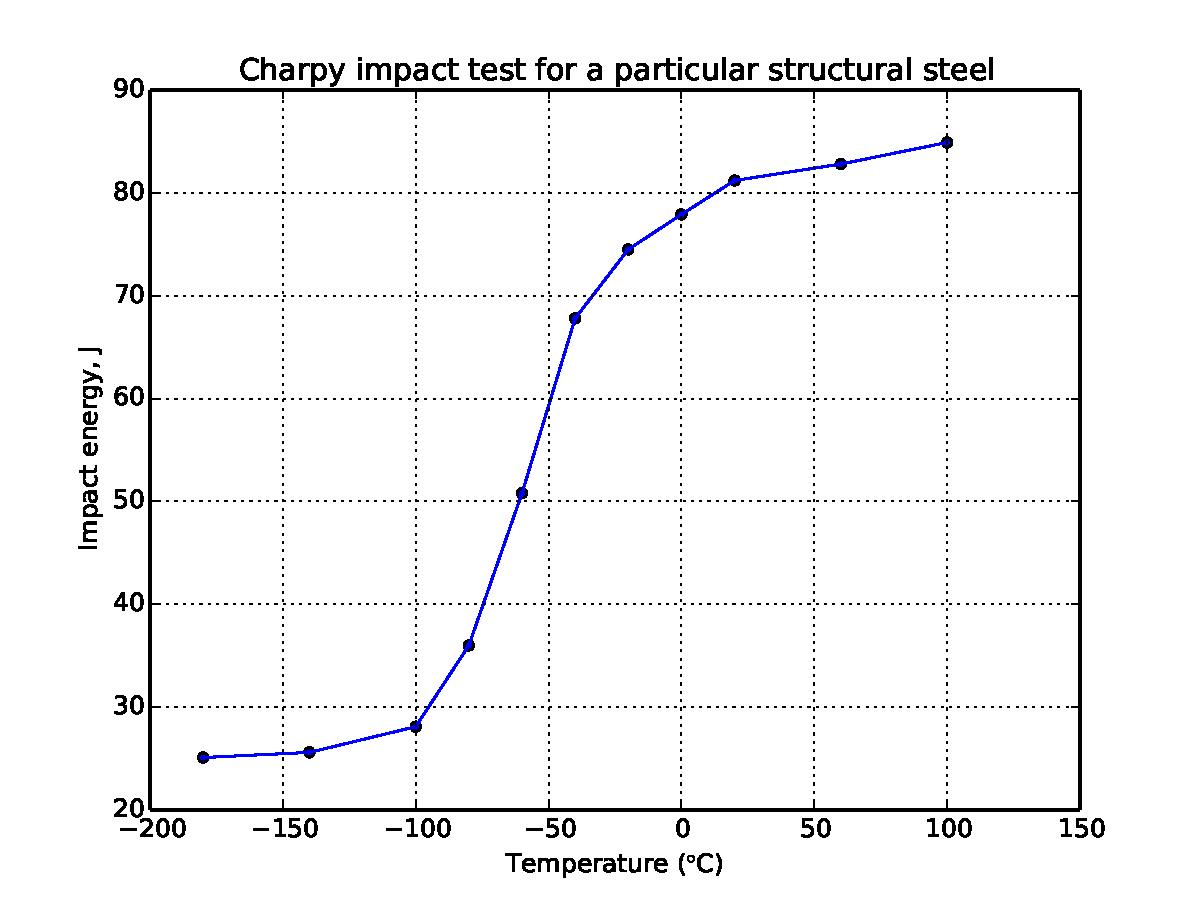
\includegraphics[width=350pt]{p2.pdf}
\caption{}
\end{figure}

\textbf{(b)} First take the average of the highest and lowest impact energies.

\begin{align*}
\frac{84.9 + 25.1}{2} = 55.0 J
\end{align*}

Looking at the graph above, an impact energy of 55 J corresponds to about -55$\degree$C ductile-to-brittle temperature.

\begin{problem}{8.6}
Generate a design plot similar to Figure 8-6 for a pressure vessel steel with Y.S. = 1000 MPa and $\text{K}_{\text{IC}}$ = 170 MPa$\sqrt{m}$.  For convenience, use the logarithmic scale for flaw size and cover a range of flaw sizes from 0.1 to 100 mm. 
\end{problem}

The red lines shows the critical flaw size. Using a yield strength of 1000MPa, a flaw size of 9.2 mm was calculated.

\begin{figure}[H]
\centering
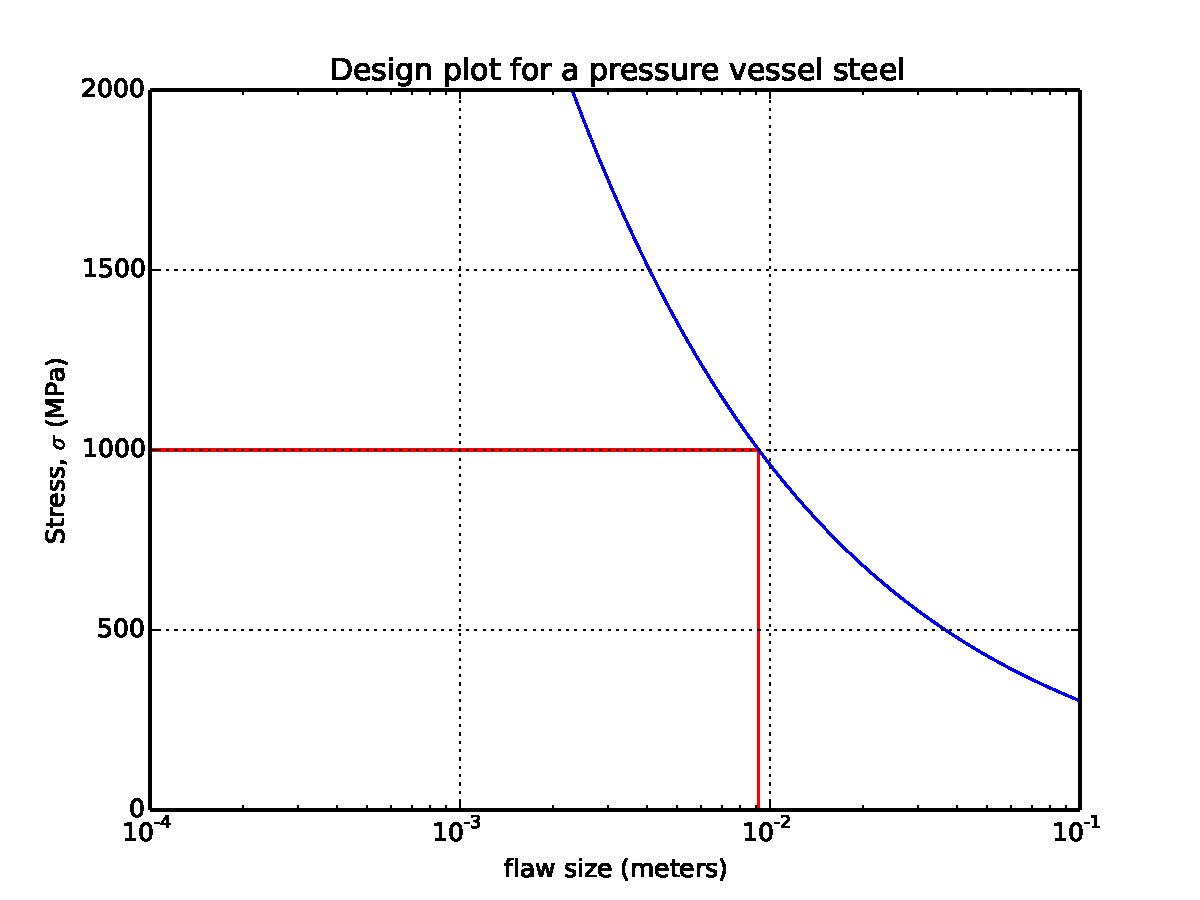
\includegraphics[width=350pt]{p3.pdf}
\caption{the red line indicates the critical flaw size at 1000 MPa stress. The critical flaw size is about 9.2 mm}
\end{figure}

\begin{problem}{8.25}
The application of a C11000 copper wire in a control circuit design will involve cyclic loading for extended periods at the elevated temperatures of a production plant.  Use the data of Figure 8.15b to specify an upper temperature limit to ensure a fatigue strength of at least 100 MPa for a stress life of $10^7$ cycles.
\end{problem}

Looking at figure 8.15, $10^7$ corresponds to three various temperature curves at different fatigues. We can make a plot of the fatigue vs temperature with these 3 lines and estimate what temperature a fatigue of 100 MPa would occur at.
\begin{figure}[H]
\centering
\begin{tabular}{c | c}
temperature ($\degree$C) & fatigue strength (MPa) \\ \hline
100 & 95 \\ \hline
65 & 125 \\ \hline
21 & 135 \\ \hline
\end{tabular}
\end{figure}

\begin{figure}[H]
\centering
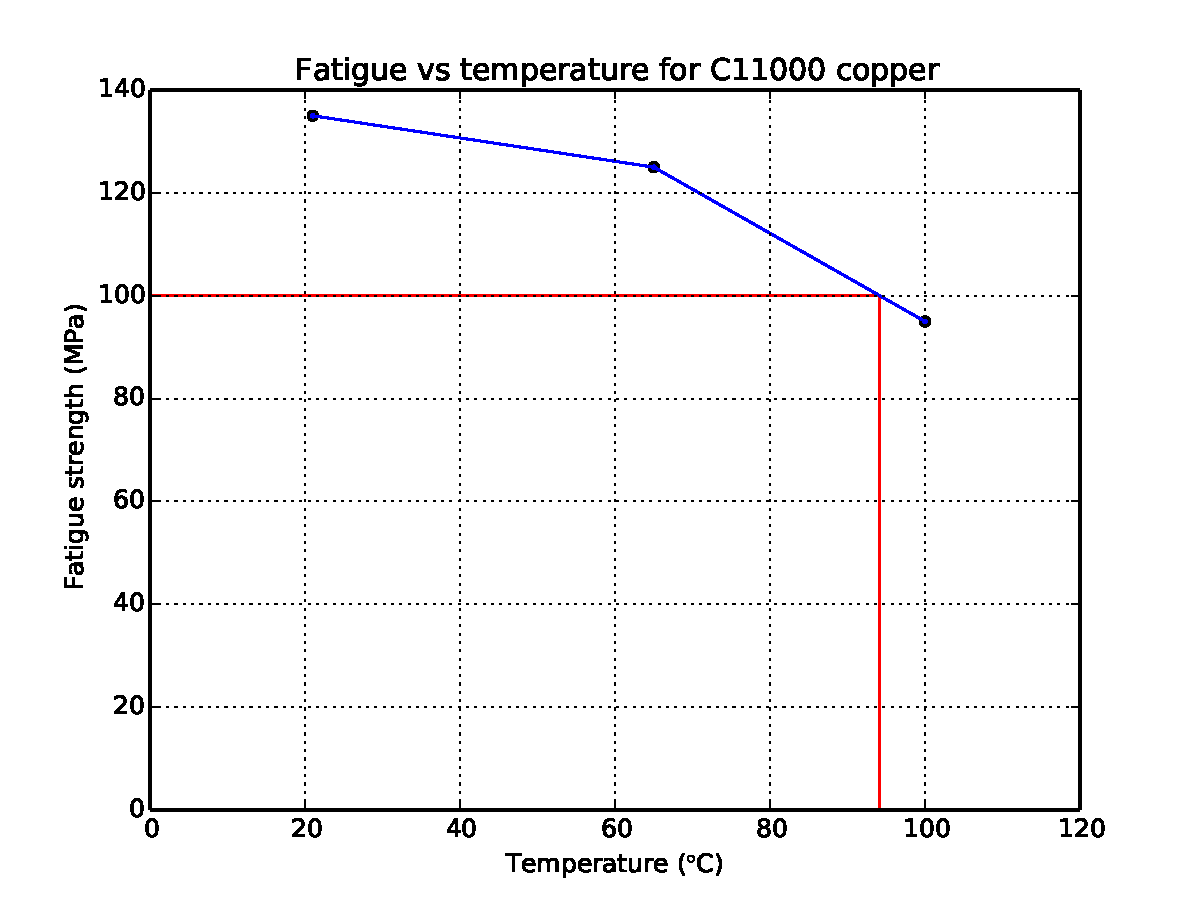
\includegraphics[width=350pt]{p4.pdf}
\caption{red line corresponds to a fatigue of 100 MPa and a temperature of about 93$\degree$C.}
\end{figure}

Using the above graph, we can now see exactly where a fatigue of 100 MPa lies. The red line indicates that a fatigue of 100 MPa corresponds to a temperature of about 94$\degree$C.

\begin{problem}{8.31}
A small pressure vessel is fabricated from an acetal polymer.  The stress in the vessel wall is,
\begin{centering}
\begin{equation}
\sigma = \frac{pr}{2t}
\end{equation}
\end{centering}
where p is the internal pressure, r the outer radius of the sphere, and t the wall thickness.  For the vessel in question, r = 30 mm and t = 2 mm.  What is the maximum permissible internal pressure for this design if the application is at room temperature and the wall stress is only tensile (due to internal pressurizations that will occur no more than $10^6$ times)?  (See Figure 8-21 for relevant data.) 
\end{problem}

Looking at figure 8.21 [1], we see that at a tensile stress only line at $10^6$ cycles corresponds to a temperature of 23$\degree$C. Room temperature in our case is 21$\degree$. So if we move slightly above the 23$\degree$C line we see that this corresponds to a stress of about 50 MPa, $\sigma = 50$MPa. We also know that thickness $t = 2$mm, and radius $r = 30$mm; this is enough for us to figure out the pressure inside the vessel. 
\begin{align*}
\sigma = \frac{pr}{2t} \Rightarrow p = \frac{2t\sigma}{r} = \frac{2*2\text{mm}*50\text{MPa}}{30\text{mm}} = \frac{20}{3}\text{MPa} = 6.67\text{MPa}
\end{align*}
\section{References}
\begin{enumerate}
\item James F. Shackelford, Introduction to Materials Science for Engineers, Seventh Edition, Pearson Higher Education, Inc., Upper Saddle River, New Jersey (2009).
\end{enumerate}




% --------------------------------------------------------------
%     You don't have to mess with anything below this line.
% --------------------------------------------------------------
 
\end{document}
